\documentclass{article}

% if you need to pass options to natbib, use, e.g.:
%     \PassOptionsToPackage{numbers, compress}{natbib}
% before loading neurips_2021

% ready for submission
\usepackage[final]{neurips_2021}

% to compile a preprint version, e.g., for submission to arXiv, add add the
% [preprint] option:
%     \usepackage[preprint]{neurips_2021}

% to compile a camera-ready version, add the [final] option, e.g.:
%     \usepackage[final]{neurips_2021}

% to avoid loading the natbib package, add option nonatbib:
%    \usepackage[nonatbib]{neurips_2021}

\usepackage[utf8]{inputenc} % allow utf-8 input
\usepackage[T1]{fontenc}    % use 8-bit T1 fonts
\usepackage{hyperref}       % hyperlinks
\usepackage{url}            % simple URL typesetting
\usepackage{booktabs}       % professional-quality tables
\usepackage{amsfonts}       % blackboard math symbols
\usepackage{nicefrac}       % compact symbols for 1/2, etc.
\usepackage{microtype}      % microtypography
\usepackage{xcolor}         % colors
\usepackage{amsmath}
\usepackage{verbatim}
\usepackage[mathscr]{euscript}
\usepackage{graphicx}
\title{Machine Learning, 2024 Spring\\Assignment 4}
% The \author macro works with any number of authors. There are two commands
% used to separate the names and addresses of multiple authors: \And and \AND.
%
% Using \And between authors leaves it to LaTeX to determine where to break the
% lines. Using \AND forces a line break at that point. So, if LaTeX puts 3 of 4
% authors names on the first line, and the last on the second line, try using
% \AND instead of \And before the third author name.



\begin{document}

\maketitle

\begin{abstract}

\end{abstract}

\textcolor{blue}{Problem 1}
For problem 3 in assignment 3, change your GD code to SGD and complete the tasks below:
\begin{itemize}
	\item Present your code.
    \item How to choose (mini -) batch size?
    \item How to choose learning rate?
    \item How to terminate?
    \item Demonstrate the impact of different learning rates on the accuracy of the solution. In other words, your program should  output an image similar to the image on page 34 of the Lecture 6-SGD PPT.
\end{itemize}

\textcolor{blue}{Solution:}\\
\begin{figure}[htbp]
  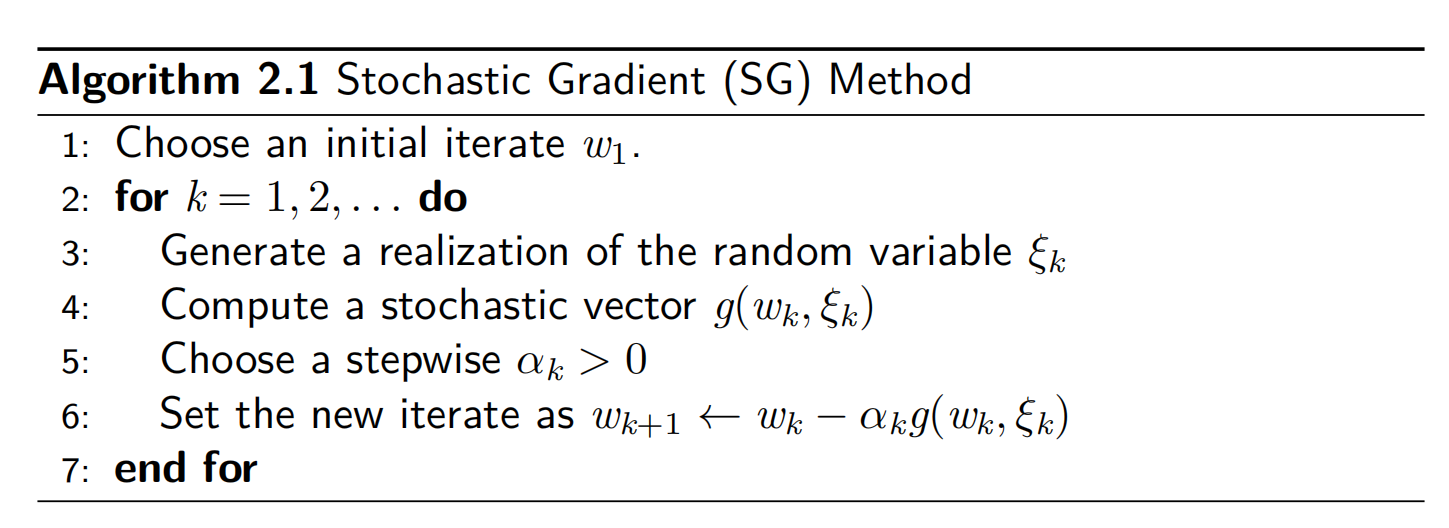
\includegraphics[width=\textwidth]{../image/alg.png}
  \caption{Stochastic Gradient Descent}
\label{fig:SGD}
\end{figure}

The SGD algorithm is implmented following the Pseudo code in Figure \ref{fig:SGD}.\\

0. Data preparation: The data is treated in the same way as the data in assignment 3:\\
The  `User ID' column is dropped, the `Age' and `EstimatedSalary' are separated into different intervals. At last, a bias term `$1$' is add for each input fetures.\\
And the features are normalized to make the data have zero mean and unit variance.\\
And before seperating the data, we random shuffled the total 400 data with a fixed seed in order to make sure the randomness, but could be stable reproduction.\\
The data is divided into training set, validation set, and testing set. The training set is used to train the model, and the validation set is used to evaluate the model for selecting the most suitable learning rate, and the testing set is used to evaluate the model for the final performance. 
The size of training, validation, and testing set is $240$, $80$, $80$ respectively, which is $60\%$, $20\%$, $20\%$ of the total data.

1. The code and the method to run the code are all in the folder `code'.

2. The mini-batch size is set to be $1$ as we are applying the stochastic gradient descent.\\
And the diction is set to be $-\nabla $:


3. The learning rate $\eta$ is tried with the following values: $0.08, 0.04, 0.02, 0.01, 0.005, 0.0025$.\\
From the results show in Figure \ref{fig:learning_rate}, we can see that the learning rate $\eta = 0.05$ has the best accuracy on the validation set. So we take the $\eta=0.05$ as the final learning rate to test on the testing set.

4. The termination condition is chosen by reaching the number of iterations: $100000$, which is large enough to make the loss converge.

5. The impact of different learning rates on the accuracy of the solution is shown in Figure \ref{fig:learning_rate}. And we can see that in the suitable range, the loss is convergence to lower value as the learning rate get smaller, which suits the regular to the image on page $34$ of the Lecture $6$-SGD PPT.\\
But we can also notice that if the learning rate is too small($\eta=0.0025$), the loss will converge to a non-optimal value. Perhaps this is because the learning rate is too small and unsuitable for the model to learn the data.\\

And the Figure \ref{fig:learning_rate} is xxxxxx.\\

% \begin{figure}[htbp]
%   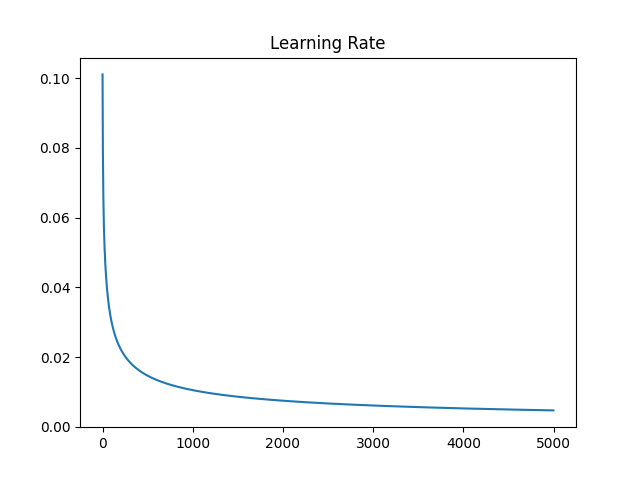
\includegraphics[width=0.5\textwidth]{../image/learning_rate.png}
%   \caption{Impact of different learning rates on the accuracy of the solution}
% \label{fig:learning_rate}
% \end{figure}














\end{document}